\chapter{Comunicación con la cámara}
\label{chap:Comunicacion con la camara}
\Abstract{En este anexo se desarrollará la conexión con la cámara Intel realsense D435}
Para el desarrollo de este proyecto se ha decidido emplear la cámara intel Realsense D435 \citep{IntelD435} ya que dispone de todos los sensores necesarios, tiene buenas prestaciones y se ha desarrollado un wrapper para permitir la conexión directa a través de MATLAB.

\begin{figure}[ht]  %Camara
	\centering
	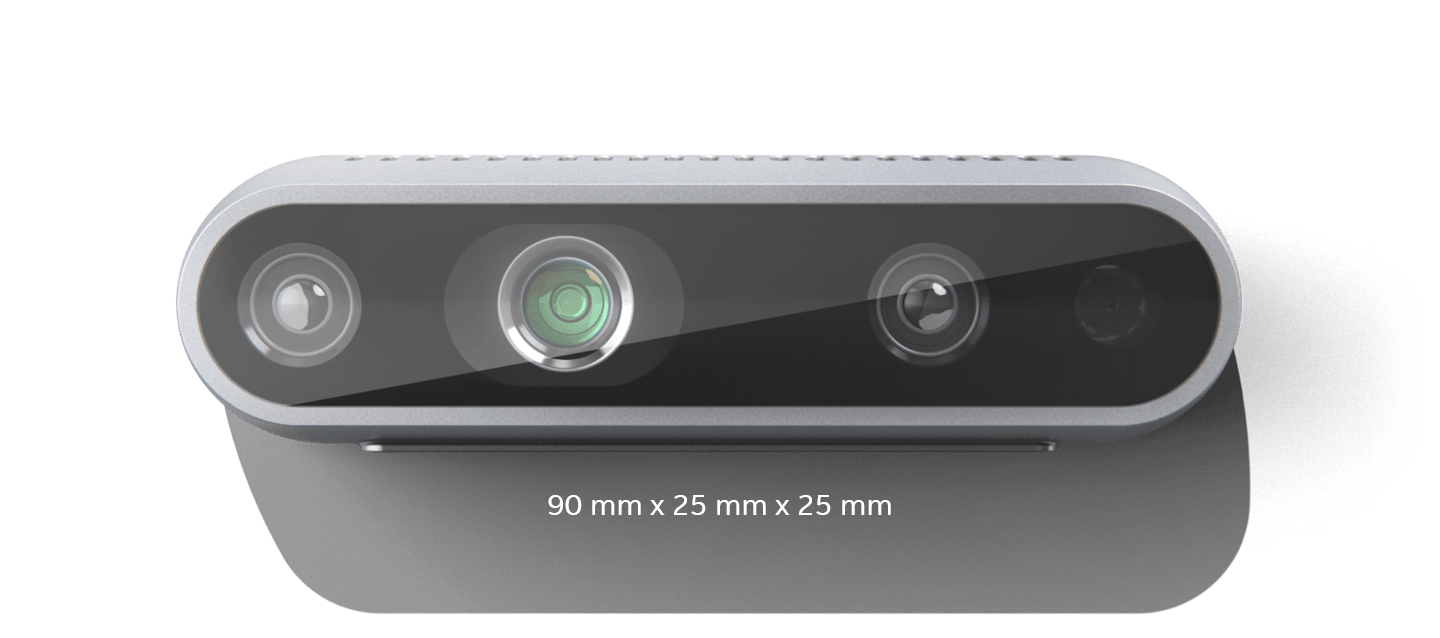
\includegraphics[width=0.95\textwidth]{Comunicacion con la camara/camara.png}
	\caption[Cámara Intel Realsense D435]{Cámara Intel Realsense D435 \citep{IntelD435}}
	\label{fig:camara}
\end{figure}

Para la conexión con la cámara se ha desarrollado una clase en MATLAB de forma que el usuario pueda acceder a todas las funciones necesarias de forma cómoda y simple sin necesidad de entender como funciona internamente. La clase ha sido creada como una herencia de la clase pipeline del wrapper de MATLAB. Pipeline se encarga de establecer la conexión entre la cámara y MATLAB y al crear nuestra clase como herencia de pipeline, nos permite tener acceso a todas las configuraciones y capacidades de pipeline y basarnos en estas para desarrollar una clase más simple e intuitiva de cara al usuario.

También se ha dado uso de la clase align del wrapper de MATLAB. Esta permite alinear la imagen de color y de profundidad de forma que ambas pasan a tener la misma resolución y tienen la misma perspectiva. Este paso es clave para mejorar la precisión del sistema ya que es la única forma de saber con certeza donde se encuentran las piezas detectadas en la imagen de color en la imagen de profundidad. El proceso se muestra en la \autoref{fig:camara alineamiento}.

La clase se ha denominado como camera y cuenta con un total de seis funciones.

\begin{itemize}
\item Constructor: Se ha desarrollado un constructor personalizado que permiten establecer la conexión con la cámara y establecer las opciones de funcionamiento.
\item Destructor: El destructor se ha desarrollado para que durante el proceso de destrucción de la instancia primero se corte de forma gradual la conexión con la cámara. De esta forma se evita futuros errores al intentar reconectarse a la cámara. Si no se realiza una desconexión progresiva no se podrá volver a abrir una conexión con la cámara y será necesario reiniciar MATLAB.
\item status: Comprueba la conexión con la cámara para asegurarse de que esta sigue activa y preparada para ser usada.
\item get\_images: función para la captura de ambas imágenes de color y profundidad. Devuelve la imagen de color y una imagen de profundidad con una resolución de 640x480 píxeles. La imagen de profundidad ha sido alineada con la de color.
\item get\_colour: función para la captura solo de la imagen de color. Devuelve la imagen de color con una resolución de 640x480 píxeles
\item get\_depth: función para la captura solo de la imagen de profundidad. Devuelve la imagen de profundidad alineada con la de color y con una resolución de 640x480 píxeles.
\end{itemize}

\begin{figure}[ht]  %Alineamiento de la profundidad
  \subfloat{
	\begin{minipage}[c][1\width]{0.3\textwidth}
	   \centering
	   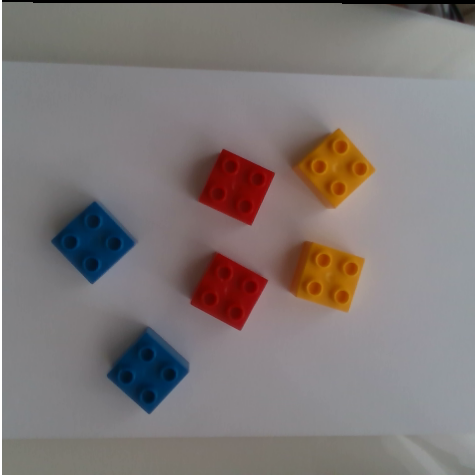
\includegraphics[width=1\textwidth]{Comunicacion con la camara/color.png}
	\end{minipage}}
  \hfill	
  \subfloat{
	\begin{minipage}[c][1\width]{0.3\textwidth}
	   \centering
	   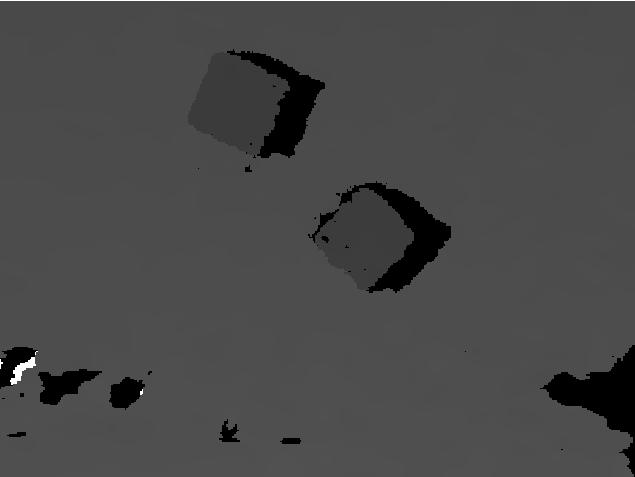
\includegraphics[width=1\textwidth]{Comunicacion con la camara/con ajuste.png}
	\end{minipage}}
  \hfill	
  \subfloat{
	\begin{minipage}[c][1\width]{0.3\textwidth}
	   \centering
	   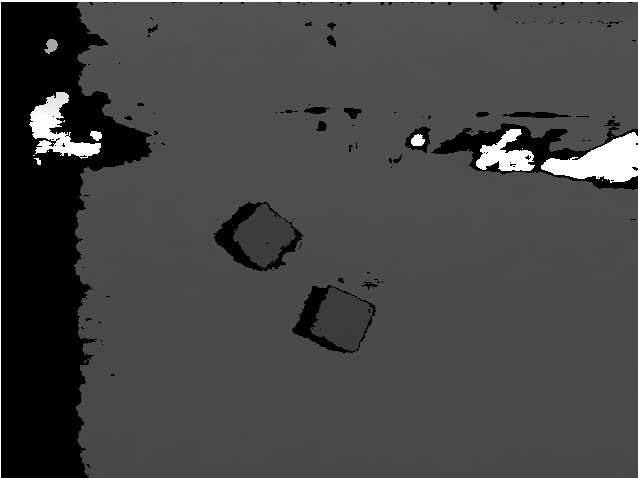
\includegraphics[width=1\textwidth]{Comunicacion con la camara/sin ajuste.png}
	\end{minipage}}
\caption[Alineamiento de imágenes de color y profundidad]{Alineamiento de las imágenes de color y profundidad tomadas con la cámara Realsense D435}
\label{fig:camara alineamiento}
\vspace{-5pt}
\end{figure}